\appendix{Ap�ndice D: Question�rio de Avalia��o e Respostas Aplicado � OntoExper-SPL}
\label{apendice:d}

Este ap�ndice apresenta o instrumento de avalia��o enviado para os especialistas de LPS e/ou Ontologias responderem citados na Se��o 2.5.

\begin{figure}[H]
	\centering					
    {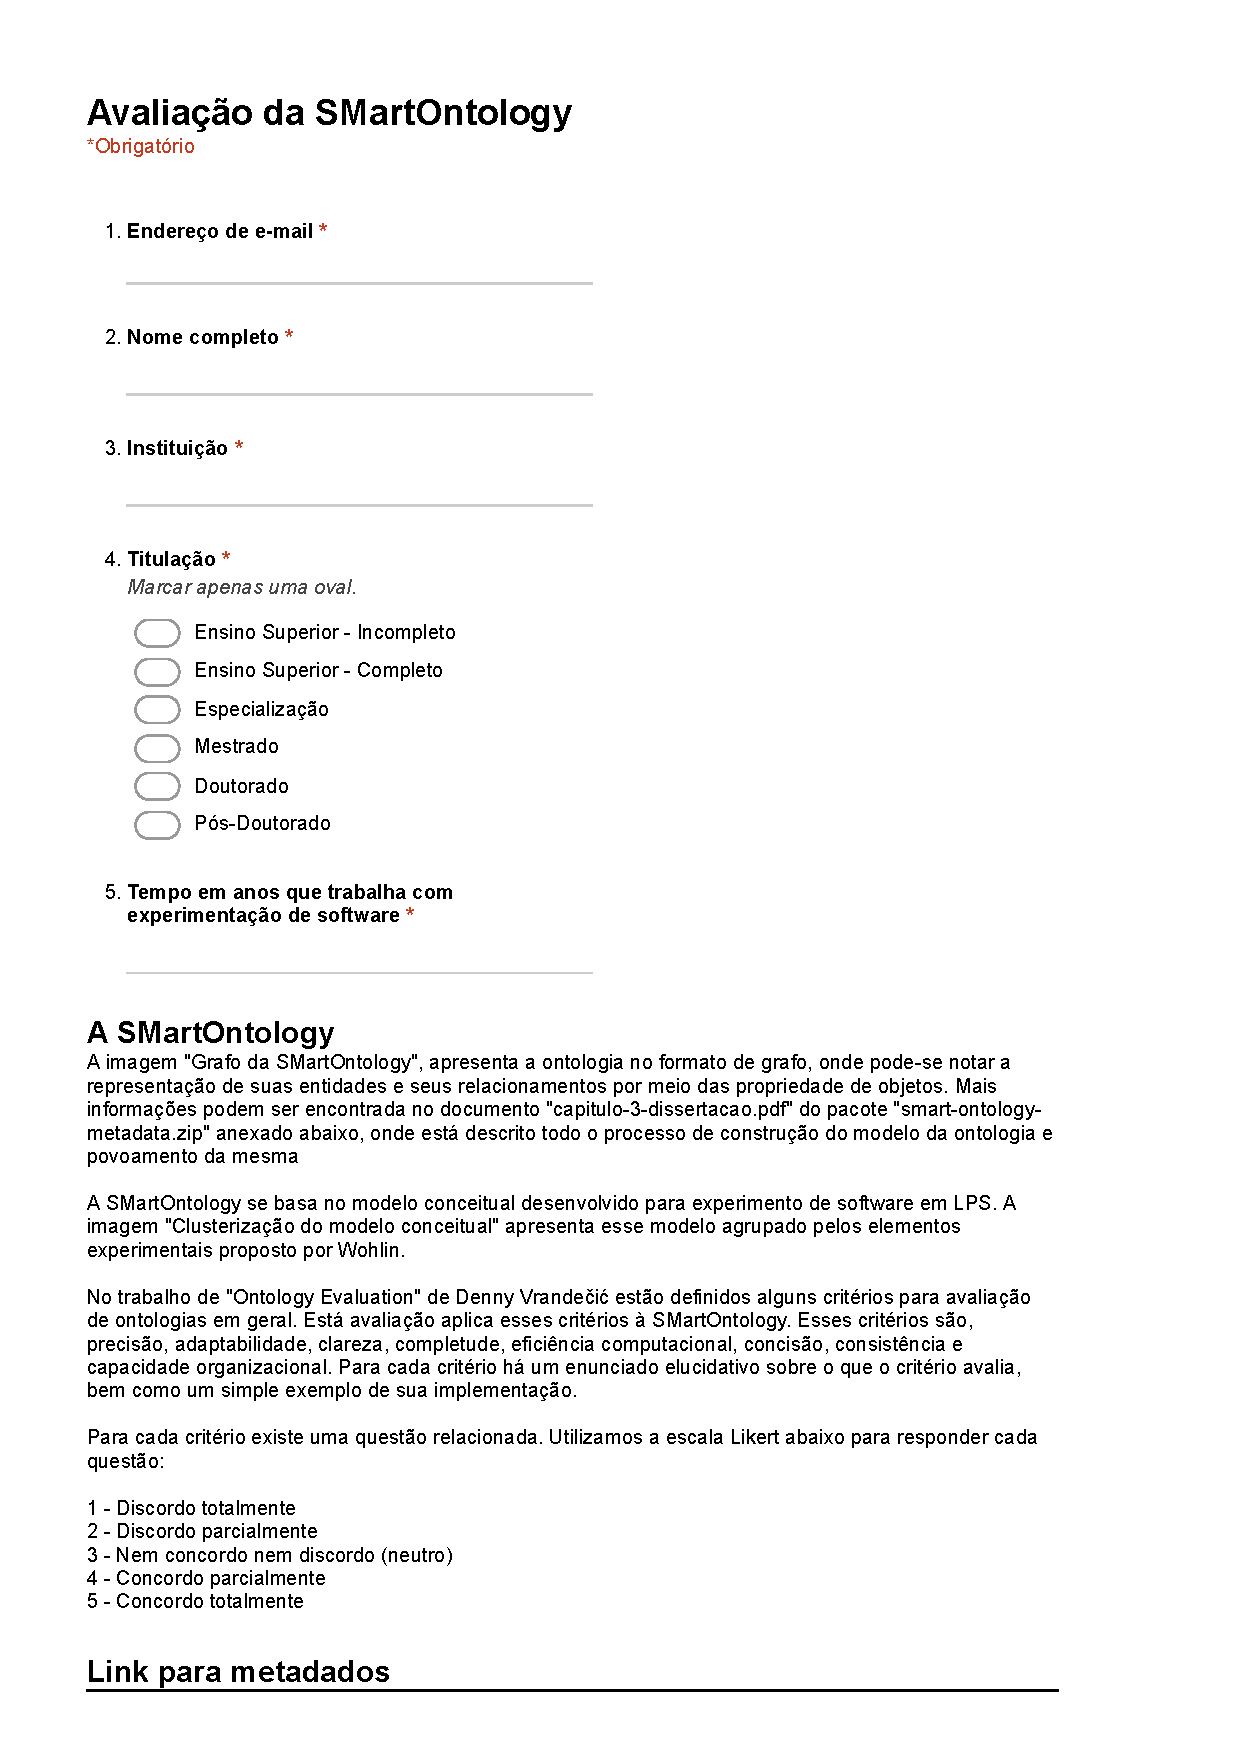
\includegraphics[scale=.45]{avaliacao-google-forms-page1.pdf}}
	\caption{Instrumento de Avalia��o pagina 1}
	\label{fig:frequencia-likert}
\end{figure}
\begin{figure}[H]
	\centering					
	{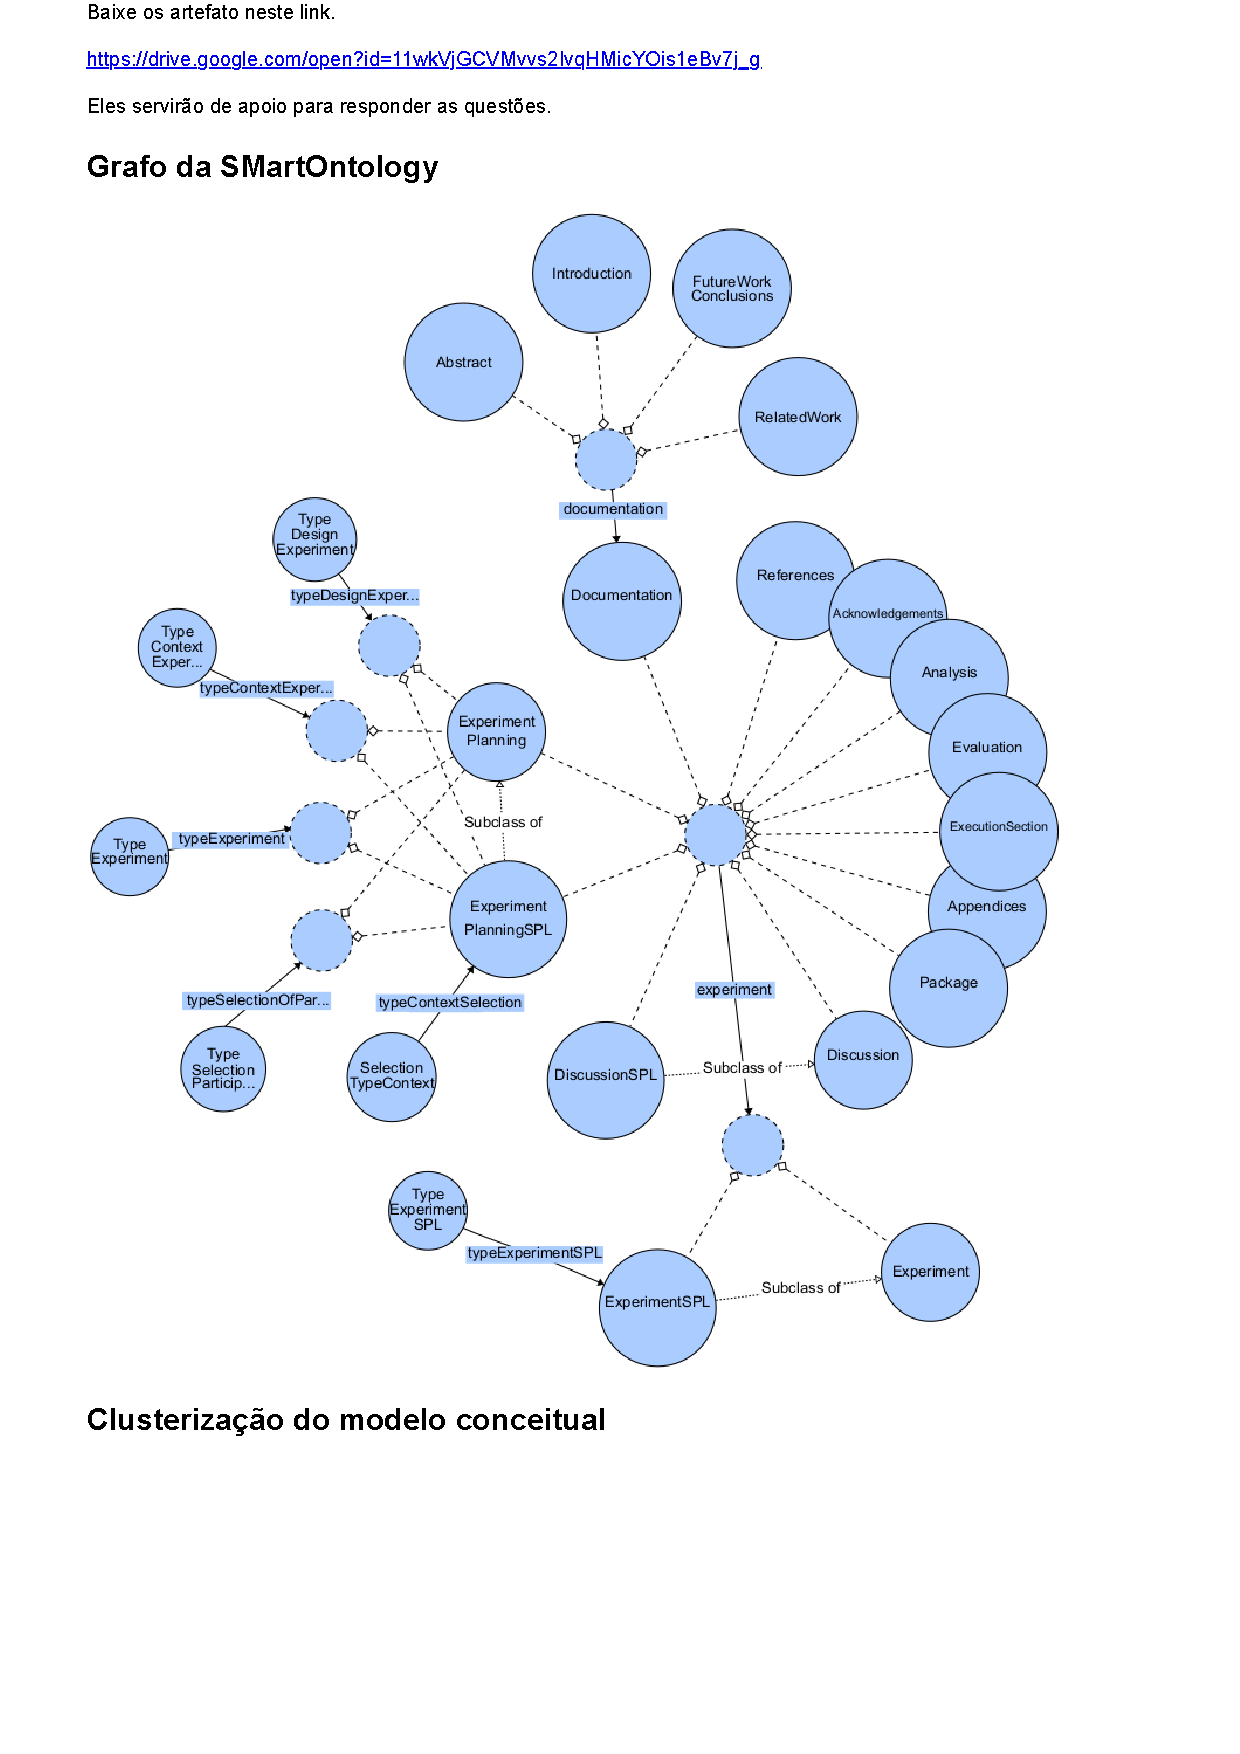
\includegraphics[scale=.7]{avaliacao-google-forms-page2.pdf}}
	\caption{Instrumento de Avalia��o pagina 2}
	\label{fig:frequencia-likert}
\end{figure}
\begin{figure}[H]
	\centering					
	{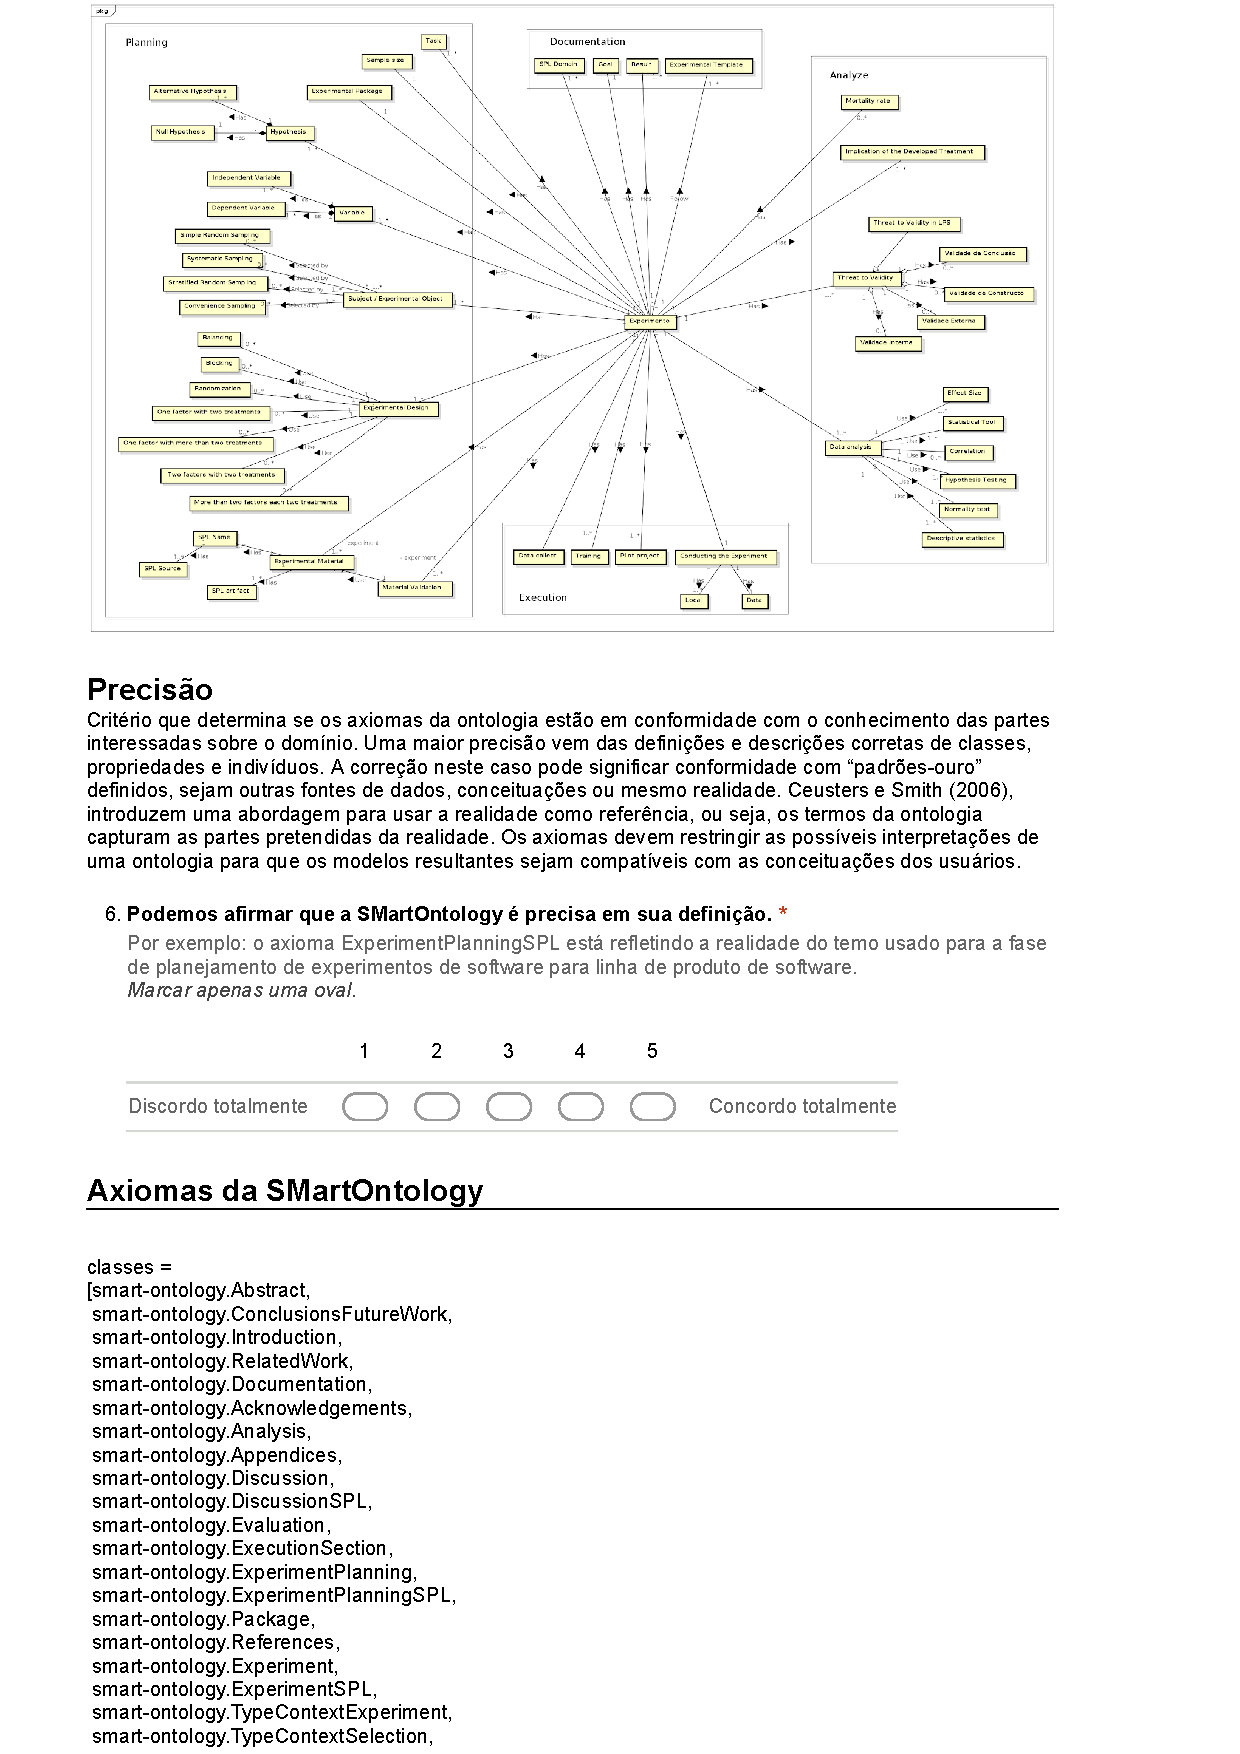
\includegraphics[scale=.7]{avaliacao-google-forms-page3.pdf}}
	\caption{Instrumento de Avalia��o pagina 3}
	\label{fig:frequencia-likert}
\end{figure}
\begin{figure}[H]
	\centering					
	{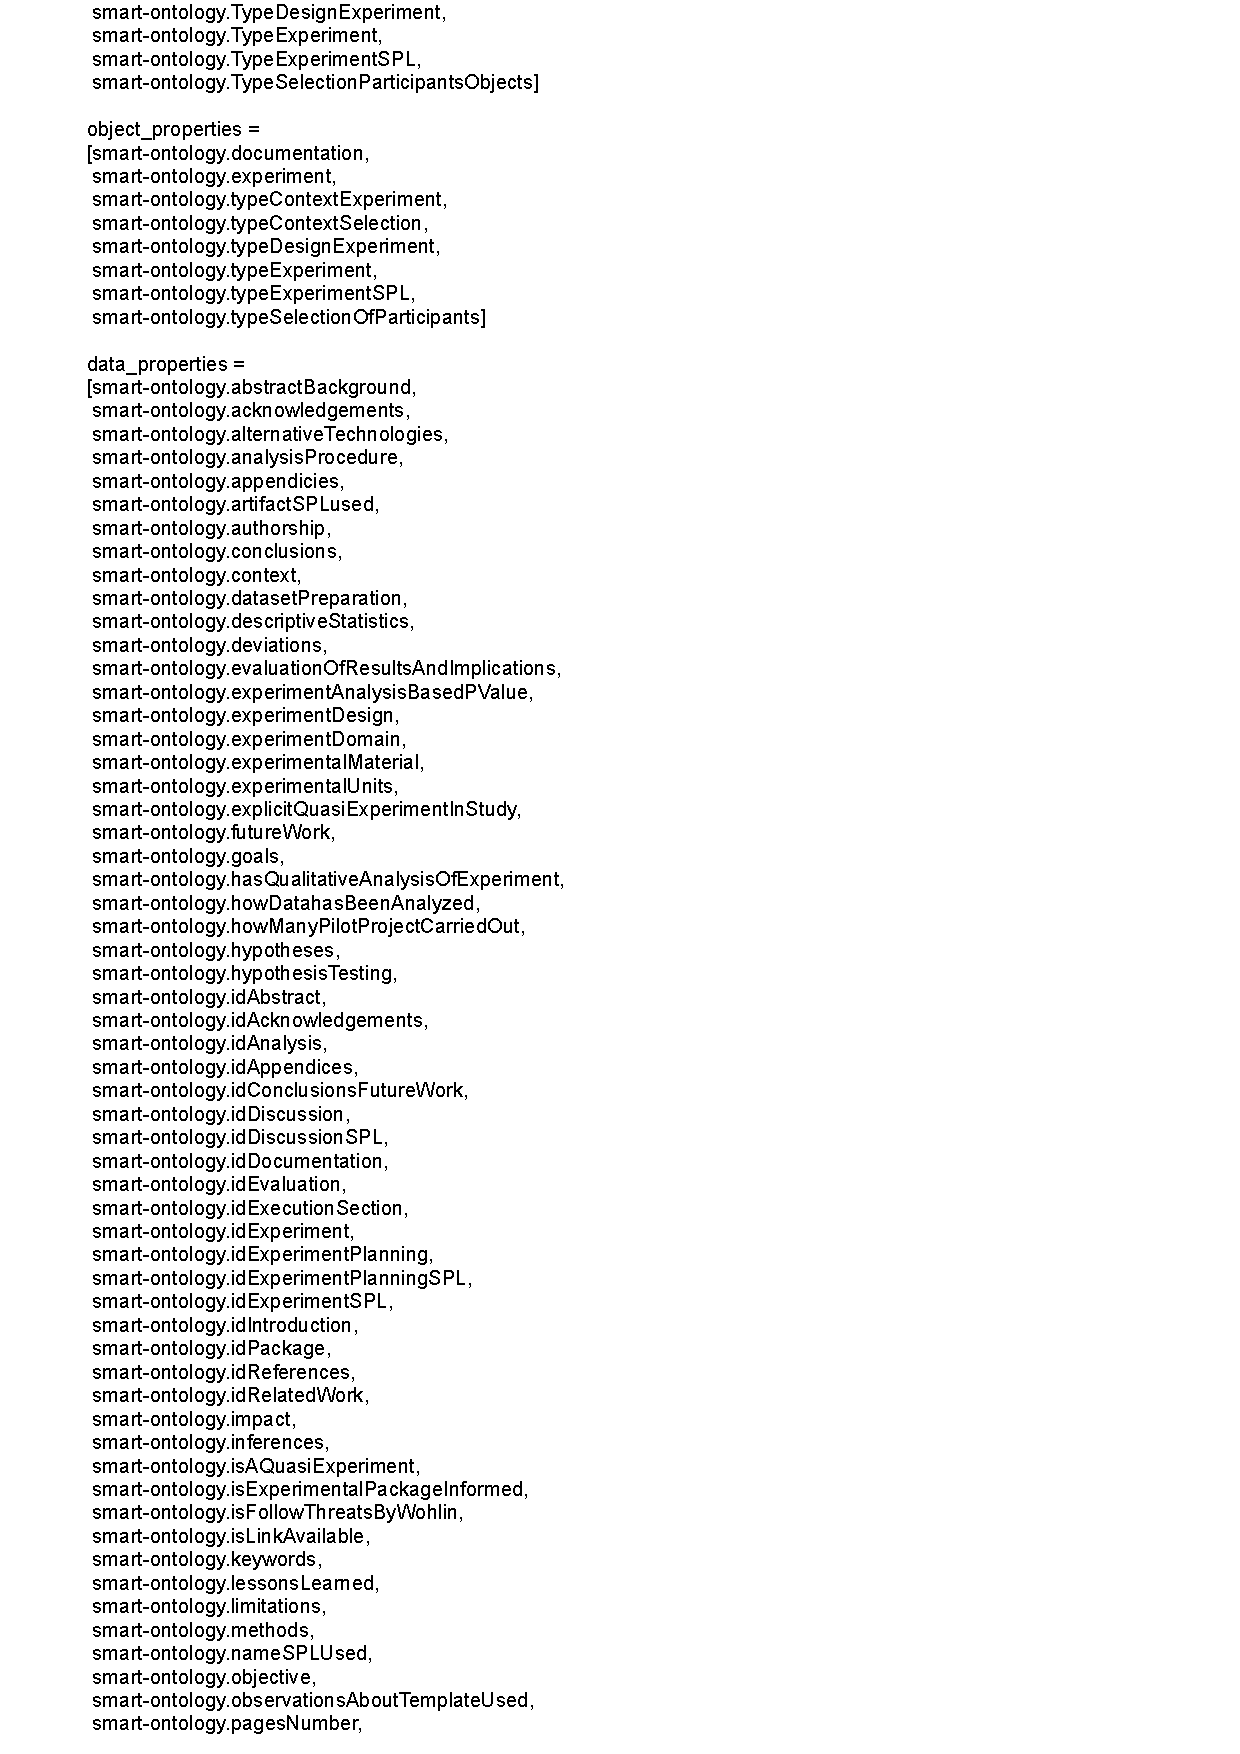
\includegraphics[scale=.7]{avaliacao-google-forms-page4.pdf}}
	\caption{Instrumento de Avalia��o pagina 4}
	\label{fig:frequencia-likert}
\end{figure}
\begin{figure}[H]
	\centering					
	{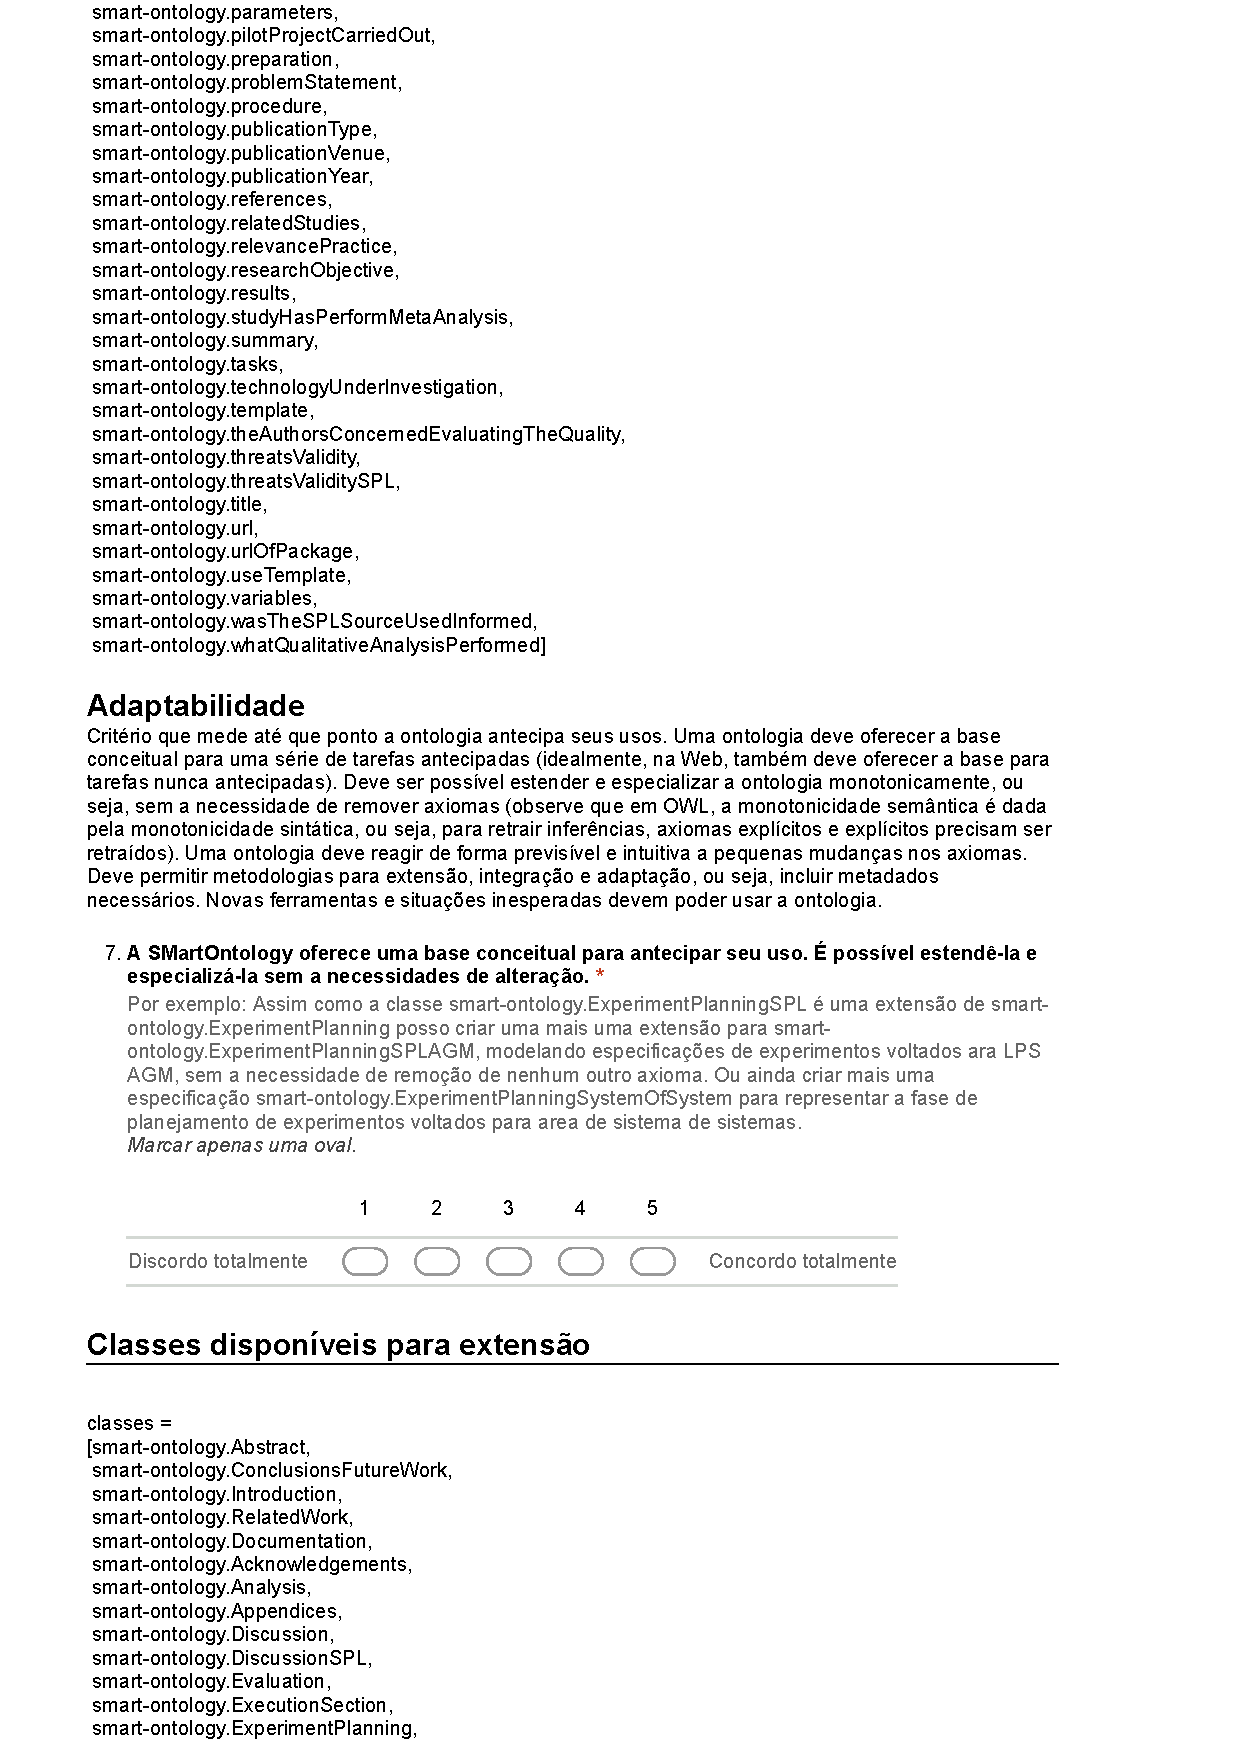
\includegraphics[scale=.7]{avaliacao-google-forms-page5.pdf}}
	\caption{Instrumento de Avalia��o pagina 5}
	\label{fig:frequencia-likert}
\end{figure}
\begin{figure}[H]
	\centering					
	{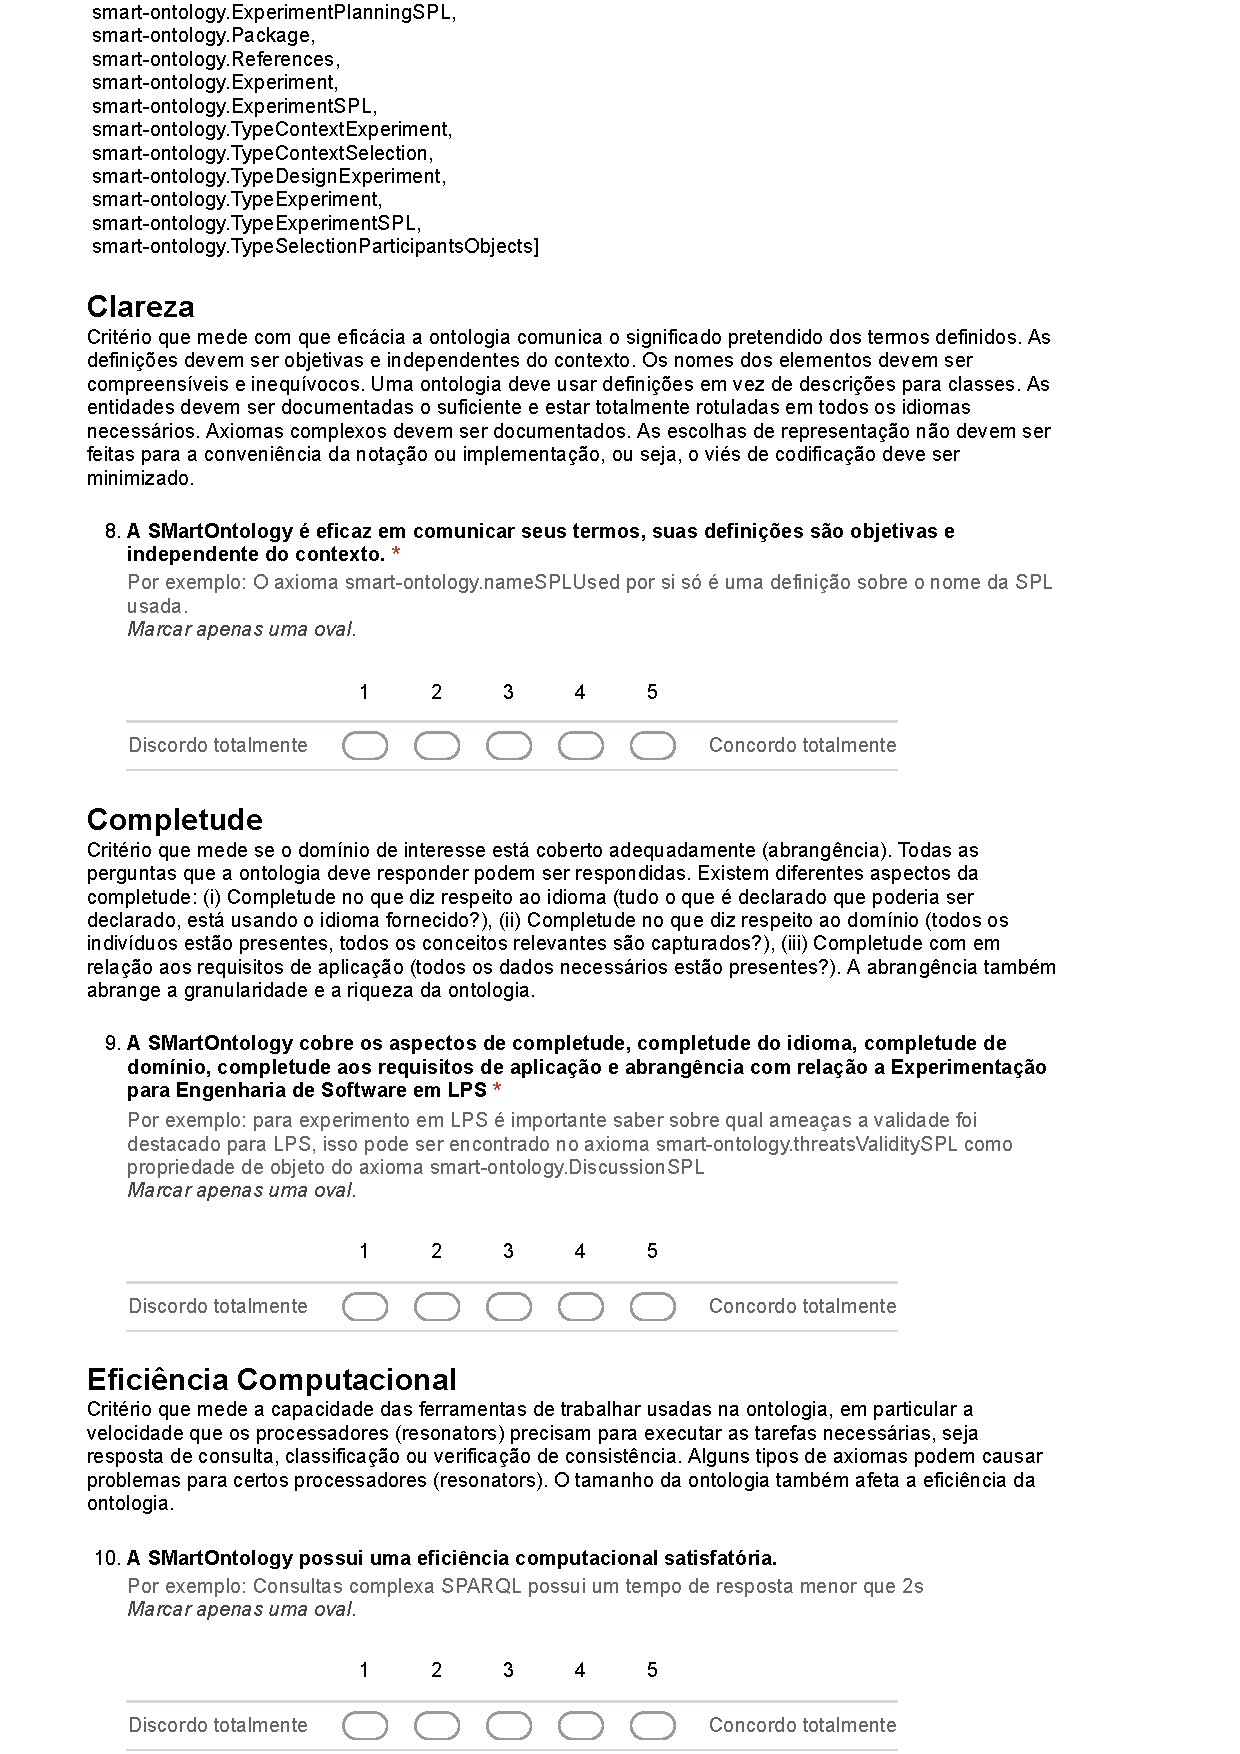
\includegraphics[scale=.7]{avaliacao-google-forms-page6.pdf}}
	\caption{Instrumento de Avalia��o pagina 6}
	\label{fig:frequencia-likert}
\end{figure}
\begin{figure}[H]
	\centering					
	{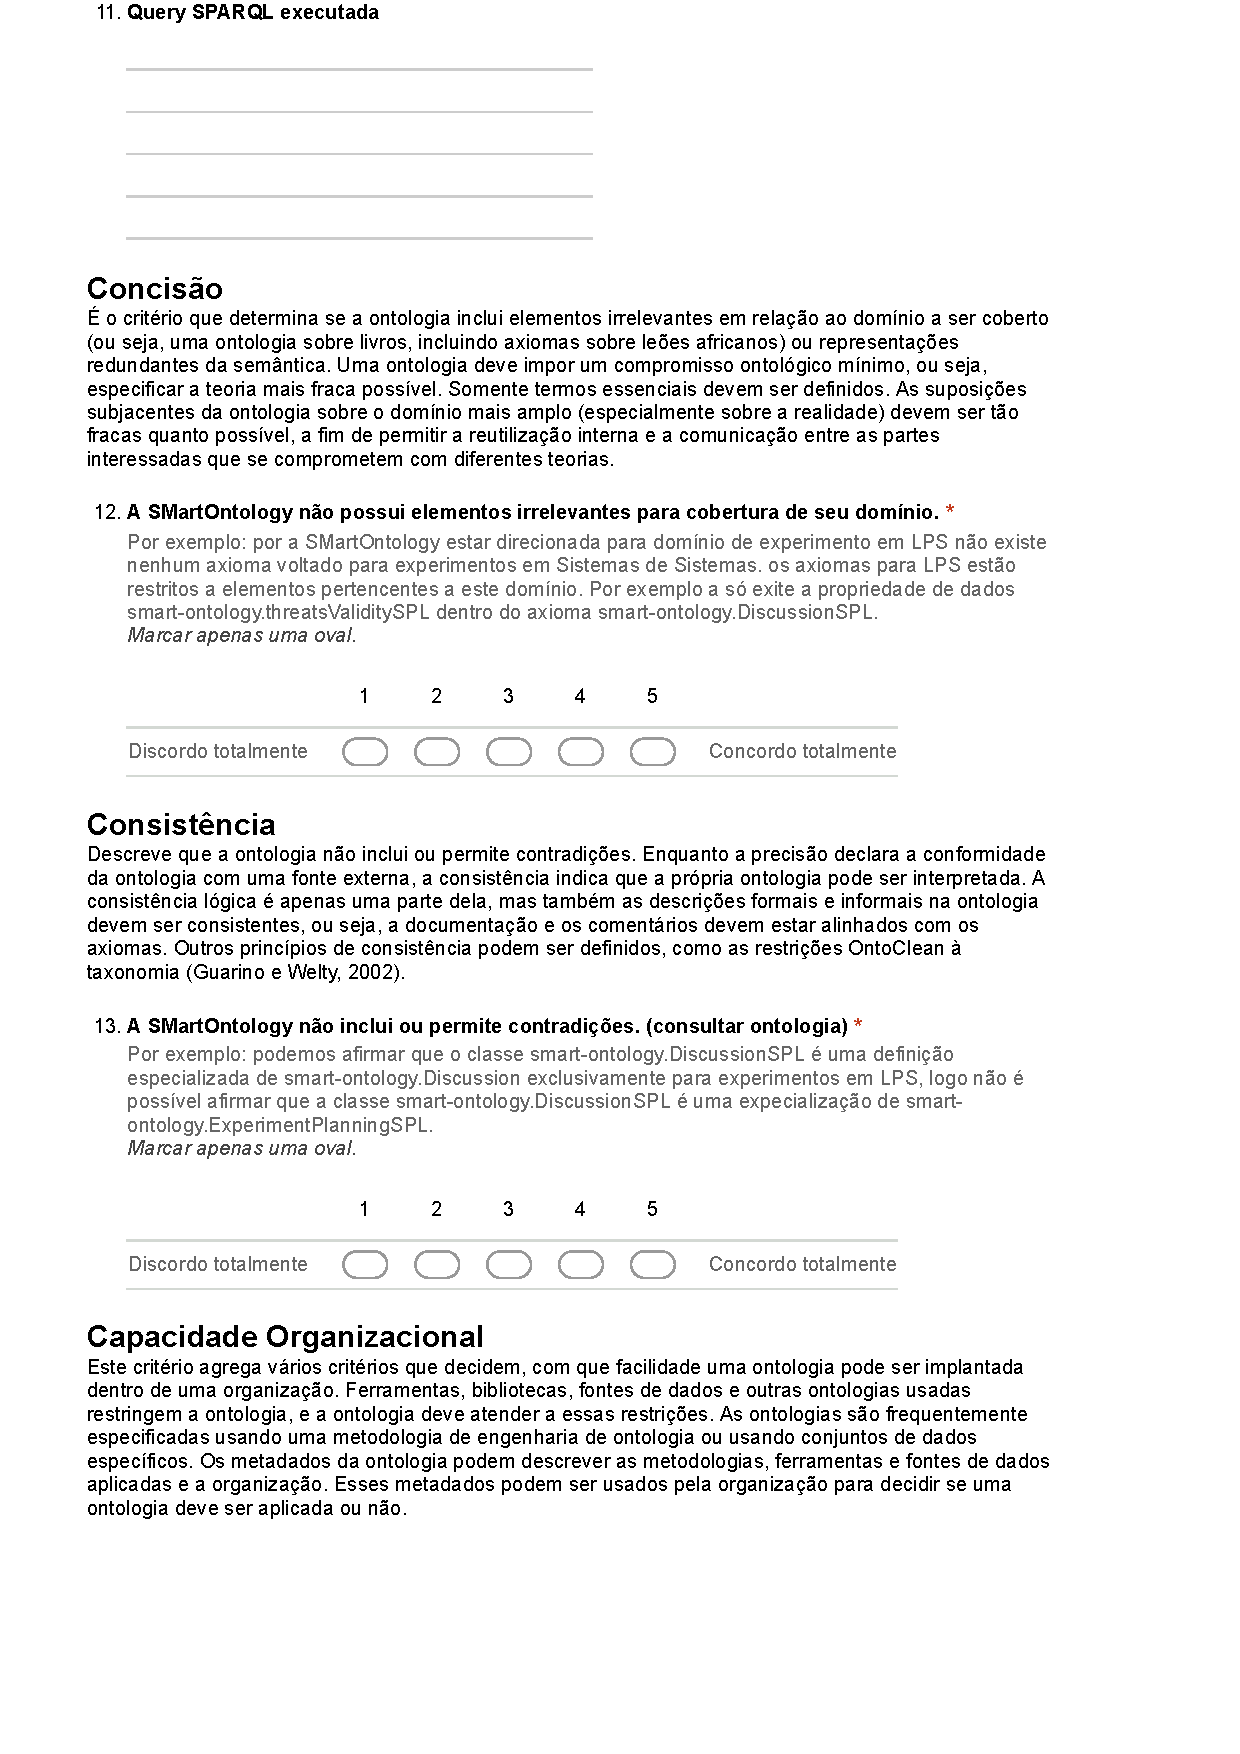
\includegraphics[scale=.7]{avaliacao-google-forms-page7.pdf}}
	\caption{Instrumento de Avalia��o pagina 7}
	\label{fig:frequencia-likert}
\end{figure}
\begin{figure}[H]
	\centering					
	{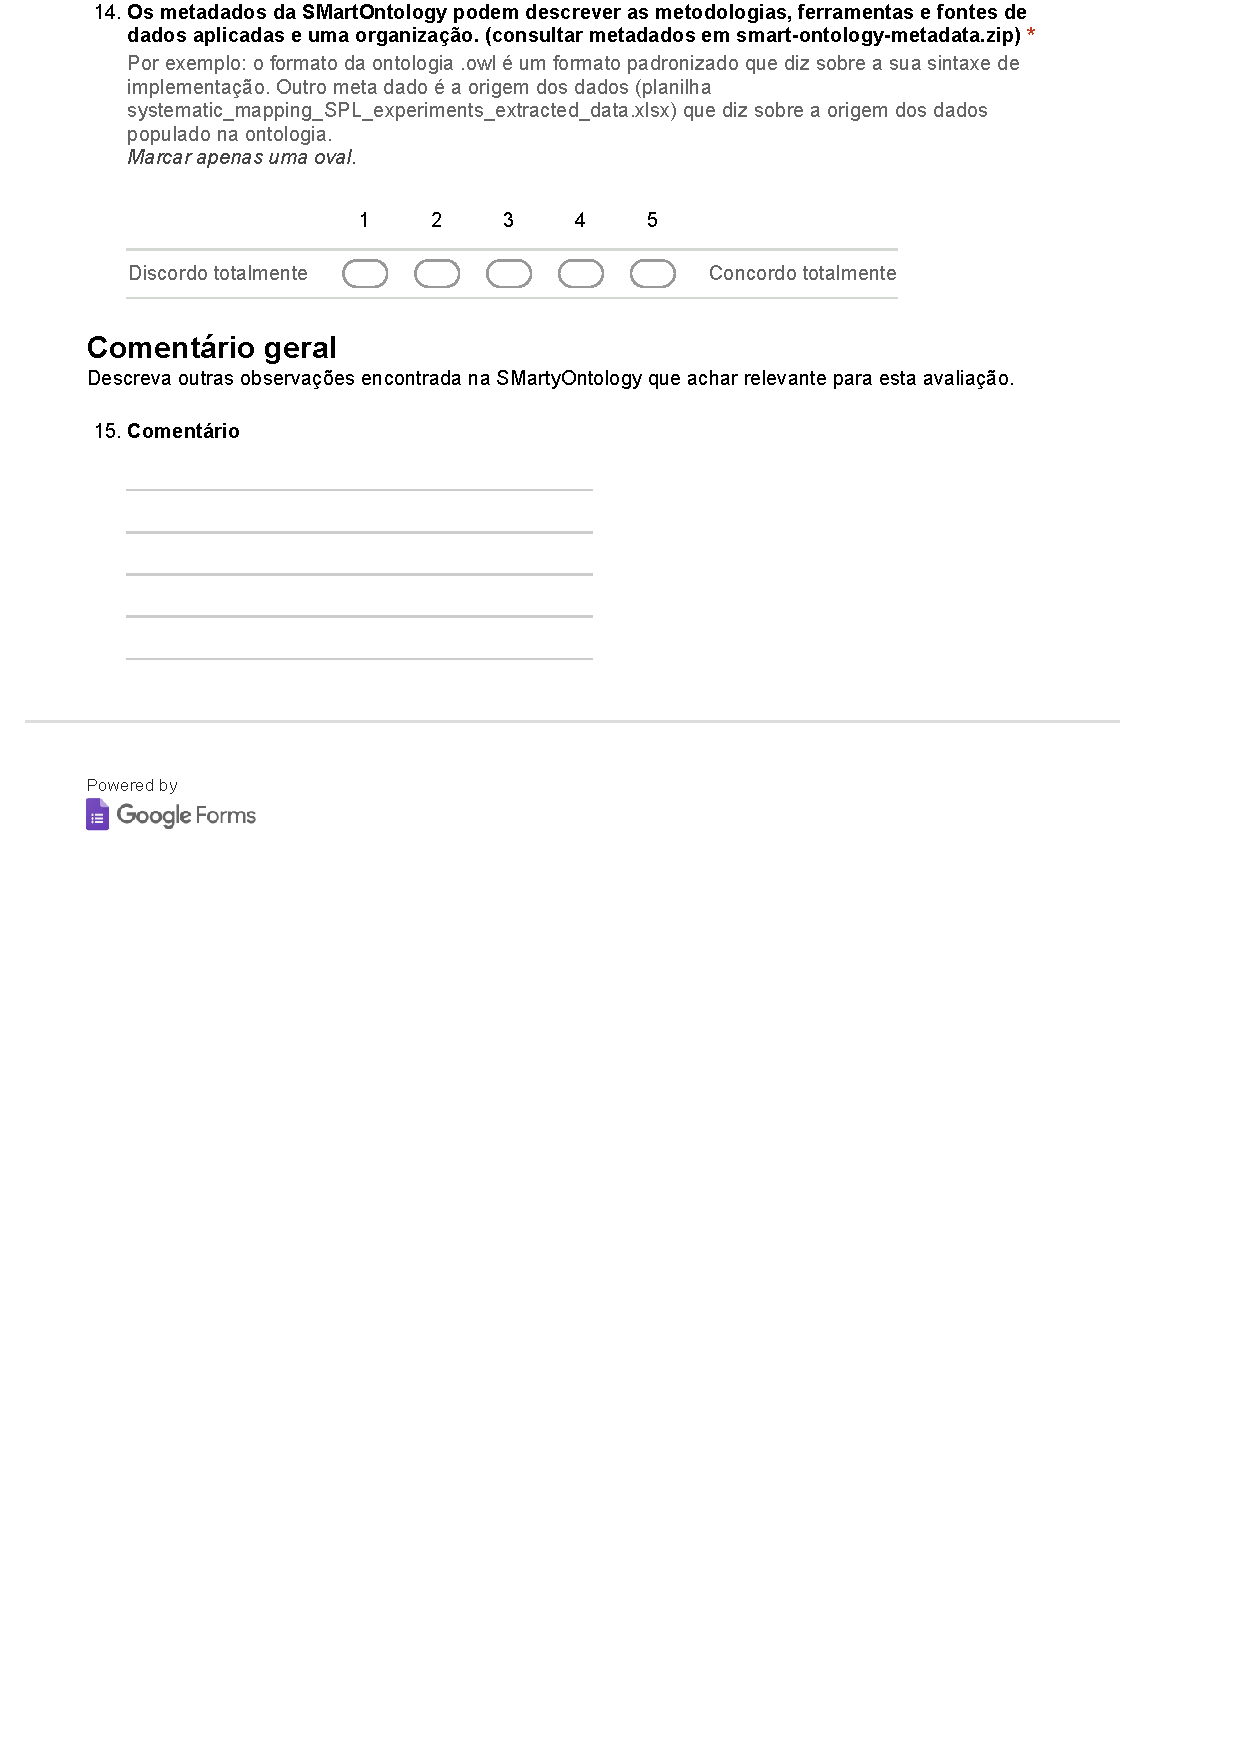
\includegraphics[scale=.7]{avaliacao-google-forms-page8.pdf}}
	\caption{Instrumento de Avalia��o pagina 8}
	\label{fig:frequencia-likert}
\end{figure}